\graphicspath{{images/}}
\newcommand{\nt}[1]{\mkern 1.5mu\overline{\mkern-1.5mu#1\mkern-1.5mu}\mkern 1.5mu}

\section*{Syntéza sekvenčného obvodu}
\subsection*{Zadanie}
Našou úlohou bolo navrhnúť obvod, ktorý strieda farby blikaním niekoľkých farebných LED.
Tlačítkom change môže užívateľ vyberať medzi niekoľkými rôznymi sekvenciami blikania.
\subsection*{Priebeh návrhu}
Najprv sa bolo potrebné rozhodnúť z koľkých LEDiek bude náš obvod tvorený, ďalej
bolo potrebné rozhodnúť o počte druhov blikania týchto lediek.
Rozhodli sme sa, že náš obvod bude schopný riadiť blikanie 5 LEDiek štyrmi druhmi 
blikania.\\
Druhy blikania boli zvolené následovne: (Tieto desiatkové číslice predstavujú päťbitové binárne
čísla - jednotlivé LEDky)\\
\begin{center}
\begin{tabular}{c c c c c c c c c}
    16 &\rightarrow  &8 &\rightarrow  &4 &\rightarrow & 2 &\rightarrow  &1 \\
    16 &\rightarrow  &1 &\rightarrow  &8 &\rightarrow & 2 &\rightarrow  &4 \\
    17 &\rightarrow &10 &\rightarrow  &4 &\rightarrow &20 &\rightarrow &21 \\
    4 &\rightarrow  &10 &\rightarrow &17 &\rightarrow &10 &\rightarrow  &4 \\
\end{tabular}
\end{center}

\noindent
Ďalej sme vytvorili graf prechodov pre automat typu MEALY pre jednotlivé stavy tohto sekvenčného obvodu.
Vyzeral približne takto:
\begin{center}
    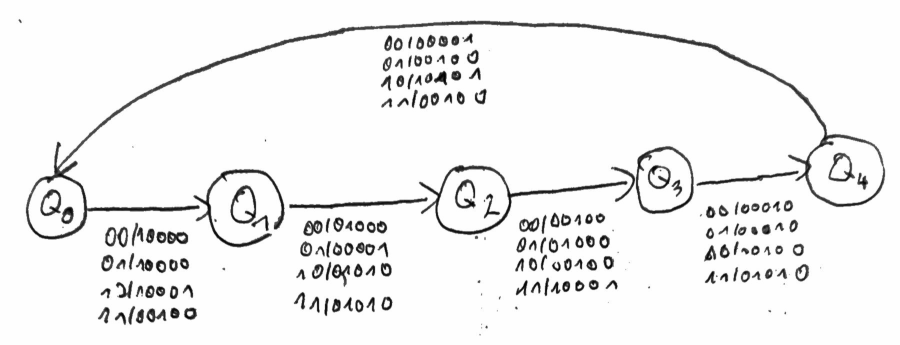
\includegraphics[width=16.2cm,height=5.4cm]{fsm_handmade.jpg}
\end{center}

\newpage
\noindent
Na kódovanie vnútorných stavov $Q_{0}..Q_{4}$ sme použili kód 1zN a na ich uchovávanie
klopné obvody D. Vďaka použitému kódovaniu môžme budiace funkcie tohto sekvenčného 
obvodu odvodiť priamo z grafu prechodov.
\begin{align*}
    D_{0}^{n+1} &= Q_{4}\\
    D_{1}^{n+1} &= Q_{0}\\
    D_{2}^{n+1} &= Q_{1}\\
    D_{3}^{n+1} &= Q_{2}\\
    D_{4}^{n+1} &= Q_{3}\\
    LA &= Q_0(\nt{I_1}\nt{I_0} + \nt{I_1}I_0 + I_1\nt{I_0}) + Q_2(I_1I_0) +
    Q_3(I_1\nt{I_0}) + Q_4(I_1\nt{I_0})\\
       &=Q_0\nt{I_1I_0} + Q_2I_1I_0 + + (Q_3 + Q_4)I_1\nt{I_0}\\
    LB &= Q_1(\nt{I_1}\nt{I_0} + I_1\nt{I_0} + I_1I_0) + Q_2(\nt{I_1}I_0) + Q_3(I_1I_0)\\
       &= Q_1\nt{\nt{I_1}I_0} + Q_2\nt{I_1}I_0 + Q_3I_1I_0\\
    LC &= Q_0(I_1I_0) + Q_2(\nt{I_1}\nt{I_0} + I_1\nt{I_0}) + Q_3(I_1\nt{I_0}) +
    Q_4(\nt{I_1}I_0 + I_1\nt{I_0} + I_1I_0)\\
       &= Q_0I_1I_0 + Q_2\nt{I_0} + Q_3I_1\nt{I_0} + Q_4\nt{\nt{I_1}\nt{I_0}}\\
    LD &= Q_1(I_1\nt{I_0} + I_1I_0) + Q_3(\nt{I_1}\nt{I_0} + \nt{I_1}I_0 + I_1I_0)\\
       &= Q_1I_1 + Q_3\nt{I_1\nt{I_0}}\\
    LE &= Q_0(I_1\nt{I_0}) + Q_1(\nt{I_1}I_0) + Q_2(I_1I_0) + Q_4(\nt{I_1}\nt{I_0} +
    I_1\nt{I_0})\\
       &= Q_0I_1\nt{I_0} + Q_1\nt{I_1}I_0 + Q_2I_1I_0 + Q_4\nt{I_0}
\end{align*}
